\documentclass{standalone}
\usepackage{tikz}
\begin{document}
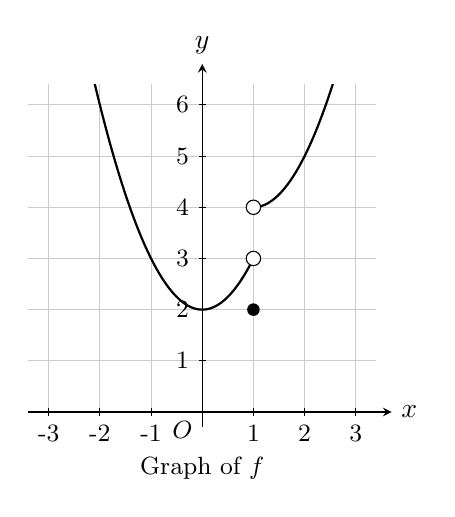
\begin{tikzpicture}[>=stealth, scale=0.65]
  % Grid
  \draw[gray!40, thin] (-3.4,0) grid (3.4,6.4);
  % Axes
  \draw[->] (-3.4,0) -- (3.7,0) node[right] {$x$};
  \draw[->] (0,-0.3) -- (0,6.8) node[above] {$y$};
  \node[below left, font=\small] at (0,0) {$O$};
  % x-axis ticks and labels
  \foreach \x in {-3,-2,-1,1,2,3} {
    \draw (\x,0.07) -- (\x,-0.07) node[below, font=\small] {\x};
  }
  % y-axis ticks and labels
  \foreach \y in {1,2,3,4,5,6} {
    \draw (0.07,\y) -- (-0.07,\y) node[left, font=\small] {\y};
  }
  % Piecewise function:
  %   left branch:  y = x^2 + 2      (x < 1), open circle at (1,3)
  %   right branch: y = (x-1)^2 + 4  (x > 1), open circle at (1,4)
  %   defined value: f(1) = 2, filled dot at (1,2)
  \begin{scope}
    \clip (-3.4,0) rectangle (3.4,6.4);
    \draw[thick, samples=100, domain=-2.3:1] plot (\x, {\x*\x + 2});
    \draw[thick, samples=100, domain=1:2.7] plot (\x, {(\x-1)*(\x-1) + 4});
  \end{scope}
  % Open circles (limit values)
  \draw[fill=white, draw=black] (1,3) circle (4pt);
  \draw[fill=white, draw=black] (1,4) circle (4pt);
  % Filled dot (defined value)
  \fill[black] (1,2) circle (3.5pt);
  % Caption
  \node[font=\small] at (0,-1.1) {Graph of $f$};
\end{tikzpicture}
\end{document}
